\documentclass[a4paper,11pt]{article}

\usepackage[slovene]{babel}
\usepackage[utf8]{inputenc}
\usepackage[T1]{fontenc}
\usepackage{amsmath,amssymb}
\usepackage{graphicx}
\usepackage{float}
\usepackage{caption}
\usepackage{subcaption}
\usepackage{hyperref}
\usepackage{listings}
\usepackage{xcolor}
\usepackage{geometry}
\geometry{margin=2.5cm}

\title{Vaja 1 -- Metoda nelinearnih najmanjših kvadratov}
\author{Ime in priimek: \textbf{Gašper Leskovec} \\
Predmet: Inteligentni sistemi za podporo odločanju \\
Datum: \today}
\date{}

\lstset{
  basicstyle=\ttfamily\small,
  backgroundcolor=\color{black!5},
  frame=single,
  captionpos=b,
  numbers=left,
  numberstyle=\tiny,
  breaklines=true,
  tabsize=2,
  literate={č}{{\v{c}}}1 {Č}{{\v{C}}}1
           {š}{{\v{s}}}1 {Š}{{\v{S}}}1
           {ž}{{\v{z}}}1 {Ž}{{\v{Z}}}1
}

\begin{document}

\maketitle

\section{Uvod}
V tej nalogi smo obravnavali problem določanja položaja izgubljenega mobilnega telefona na podlagi meritev razdalj do treh baznih postaj. Ker so meritve obremenjene s šumom, problema ni smiselno obravnavati kot eksaktno reševanje sistema enačb -- tri šumne krožnice se v splošnem ne sekajo v eni točki. Namesto tega problem zastavimo kot \emph{optimizacijski problem}: iščemo točko, ki se izmerjenim razdaljam ``najbolje prilega'' v smislu najmanjše vrednosti izbrane kriterijske funkcije. Za rešitev smo uporabili metodo nelinearnih najmanjših kvadratov, natančneje Levenberg--Marquardtovo (LM) metodo.

Poleg osnovne lokalizacije smo v nalogi obravnavali tri metodološka vprašanja, ki so ključna za pravilno statistično interpretacijo rezultata:
\begin{enumerate}
    \item kako v kriterijsko funkcijo vključiti \emph{varianco meritev} posameznih postaj (uteženi najmanjši kvadrati, WLS),
    \item kako pravilno izvesti LM iteracijo z logiko \emph{sprejmi/zavrni} (accept/reject), ki koraka ne sprejme brezpogojno,
    \item kako pravilno oceniti \emph{varianco ocene pozicije} -- z Monte Carlo ponovitvami neodvisnih eksperimentov, ne z varianco optimizacijske poti.
\end{enumerate}

\section{Opis naloge}
Tri bazne postaje so postavljene v ravnini na znanih koordinatah:
\begin{itemize}
    \item Bazna postaja 1: $(1,1)$
    \item Bazna postaja 2: $(10,5)$
    \item Bazna postaja 3: $(2,4)$
\end{itemize}

Vsaka bazna postaja ob klicu funkcije \texttt{ping\_stolp\_1}, \texttt{ping\_stolp\_2} oziroma \texttt{ping\_stolp\_3} vrne eno šumno meritev razdalje do telefona; vsak klic vrne drugačno vrednost.

Naloga je bila sestavljena iz treh delov:
\begin{enumerate}
    \item določitev položaja telefona pri $N=100$ meritvah na postajo, v neuteženi in uteženi izvedbi,
    \item Monte Carlo analiza vpliva števila meritev $N \in \{1,5,10,50,100\}$ na varianco končne ocene in na konvergenco,
    \item primerjava uteženega in neuteženega pristopa pri $N=100$.
\end{enumerate}
Naloga je rešena izključno z osnovnim MATLAB-om, brez uporabe toolboxov (tudi krožnice na slikah so narisane ročno s parametrizacijo $(x_c + r\cos\theta,\; y_c + r\sin\theta)$).

\section{Matematični model}

\subsection{Optimizacijski problem in kriterijska funkcija}
Naj bo neznani položaj telefona podan z vektorjem
\[
\mathbf{x} = \begin{bmatrix} x \\ y \end{bmatrix}.
\]
Če bi bile meritve točne, bi za vsako postajo veljalo $(x-x_i)^2 + (y-y_i)^2 = d_i^2$. Ker so meritve šumne, enačbe niso izpolnjene eksaktno; za vsako bazno postajo zato definiramo \emph{rezidual} (ostanek), ki pove, kako daleč je točka $(x,y)$ od izpolnitve $i$-te enačbe:
\[
F_i(x,y) = (x-x_i)^2 + (y-y_i)^2 - d_i^2,
\]
kjer sta $(x_i,y_i)$ koordinati $i$-te bazne postaje, $d_i$ pa (povprečena) izmerjena razdalja do telefona. Celoten rezidualni vektor je
\[
\mathbf{F}(x,y)=
\begin{bmatrix}
(x-x_1)^2+(y-y_1)^2-d_1^2 \\
(x-x_2)^2+(y-y_2)^2-d_2^2 \\
(x-x_3)^2+(y-y_3)^2-d_3^2
\end{bmatrix}.
\]

Optimizacijski problem se glasi: poišči $(x,y)$, ki minimizira \emph{kriterijsko funkcijo}
\begin{equation}
J(x,y) = \mathbf{F}^T \mathbf{W}\, \mathbf{F},
\label{eq:kriterij}
\end{equation}
kjer je $\mathbf{W}$ diagonalna matrika uteži. Kriterijska funkcija je torej utežena vsota kvadratov rezidualov: vsaka postaja prispeva svoj kvadrirani rezidual, pomnožen s svojo utežjo. V posebnem primeru $\mathbf{W}=\mathbf{I}$ dobimo običajne (neutežene) najmanjše kvadrate $J = \|\mathbf{F}\|^2$.

\subsection{Uteženi najmanjši kvadrati in varianca meritev}
\label{sec:wls}
Vse tri postaje niso enako zanesljive: šum meritev ima pri vsaki postaji drugačno velikost. Če iz $N$ surovih meritev $d_i^{(1)},\dots,d_i^{(N)}$ za vsako postajo poleg povprečja
\[
\bar{d}_i = \frac{1}{N}\sum_{k=1}^{N} d_i^{(k)}
\]
ocenimo še vzorčno varianco
\[
\sigma_i^2 = \frac{1}{N-1}\sum_{k=1}^{N} \left(d_i^{(k)} - \bar{d}_i\right)^2,
\]
lahko to informacijo vgradimo v kriterij~\eqref{eq:kriterij} z izbiro
\begin{equation}
\mathbf{W} = \operatorname{diag}\!\left(\frac{1}{\sigma_1^2},\; \frac{1}{\sigma_2^2},\; \frac{1}{\sigma_3^2}\right).
\label{eq:W}
\end{equation}

Zakaj je ta izbira smiselna? Intuitivno: rezidual postaje z velikim raztrosom meritev je že zaradi šuma pogosto velik, čeprav je točka $(x,y)$ pravilna -- taki postaji zato ne smemo slepo verjeti in njen prispevek h kriteriju pomnožimo z majhno utežjo $1/\sigma_i^2$. Nasprotno postaja z majhno varianco meri natančno, zato njen rezidual nosi več informacije in dobi veliko utež. Formalno ta izbira izhaja iz metode največjega verjetja: če so pogreški meritev neodvisni in normalno porazdeljeni z različnimi variancami (heteroskedastičen šum), je ocena z največjim verjetjem ravno rešitev uteženih najmanjših kvadratov z utežmi, obratno sorazmernimi z variancami. Uteženje s $1/\sigma_i^2$ poleg tega poskrbi, da so členi kriterija brezdimenzijski in medsebojno primerljivi -- vsak rezidual je normiran s ``tipično'' velikostjo svojega šuma.

\subsection{Levenberg--Marquardtova metoda z logiko sprejmi/zavrni}
\label{sec:lm}
Kriterij~\eqref{eq:kriterij} je nelinearna funkcija parametrov, zato ga minimiziramo iterativno. Jacobijeva matrika rezidualov je
\[
\mathbf{J}(x,y)=
\begin{bmatrix}
2(x-x_1) & 2(y-y_1) \\
2(x-x_2) & 2(y-y_2) \\
2(x-x_3) & 2(y-y_3)
\end{bmatrix},
\]
kandidat za korak v $k$-ti iteraciji pa je rešitev linearnega sistema
\begin{equation}
\Delta = \left(\mathbf{J}^T \mathbf{W} \mathbf{J} + \lambda \mathbf{I}\right)^{-1}\left(-\mathbf{J}^T \mathbf{W} \mathbf{F}\right).
\label{eq:step}
\end{equation}
Parameter dušenja $\lambda$ interpolira med Gauss--Newtonovo metodo (majhen $\lambda$, dolgi in ``pogumni'' koraki) in gradientnim spustom z majhnim korakom (velik $\lambda$, kratki in previdni koraki).

Ključno je, da izračunani korak $\Delta$ obravnavamo zgolj kot \emph{kandidata}, ne kot dokončno posodobitev. Enačba~\eqref{eq:step} namreč temelji na linearizaciji rezidualov okoli trenutne točke; če je korak predolg, linearizacija zunaj njene okolice ne velja več in kriterij se v novi točki lahko celo \emph{poslabša}. Metoda, ki vsak korak sprejme brezpogojno, lahko zato skače po prostoru parametrov in v neugodnih primerih divergira -- prilagajanje $\lambda$ šele \emph{po} že sprejetem slabem koraku škode ne prepreči. Pravilna LM iteracija zato deluje po logiki \emph{sprejmi/zavrni}:
\begin{enumerate}
    \item izračunaj kandidata $\mathbf{x}_{\text{new}} = \mathbf{x}_k + \Delta$ in vrednost kriterija $J(\mathbf{x}_{\text{new}})$;
    \item če je $J(\mathbf{x}_{\text{new}}) < J(\mathbf{x}_k)$: korak \textbf{sprejmi} ($\mathbf{x}_{k+1} = \mathbf{x}_{\text{new}}$), zmanjšaj $\lambda \leftarrow \lambda/10$ (linearizaciji lahko bolj zaupamo) in preveri konvergenco ($\|\Delta\| < 10^{-6}$);
    \item sicer: korak \textbf{zavrni} ($\mathbf{x}_{k+1} = \mathbf{x}_k$, položaj se ne spremeni), povečaj $\lambda \leftarrow 10\lambda$ in iz iste točke poskusi znova s krajšim, bolj dušenim korakom;
    \item varovalka: če $\lambda$ preseže $10^{10}$, se iteracija prekine z opozorilom (preprečitev neskončne zanke zavračanj).
\end{enumerate}

Pomembno je razumeti, kaj ta logika garantira in česa ne. \emph{Garantira} monotono padanje kriterija $J$ po sprejetih korakih: vrednost uteženega kvadrata rezidualov se z vsakim sprejetim korakom strogo zmanjša, zato metoda ne more ``pobegniti'' od že dosežene kakovosti rešitve. \emph{Ne garantira} pa ravne ali monotone poti samih parametrov: sprejeti korak lahko posamezno koordinato začasno odmakne od končne rešitve, če se kriterij pri tem vseeno zmanjša. Na to se vrnemo pri interpretaciji konvergenčnega grafa v razdelku~\ref{sec:rez_main}.

\subsection{Varianca poti proti Monte Carlo varianci ocene}
\label{sec:mc_teorija}
Zadnje metodološko vprašanje je, kaj sploh pomeni ``varianca pozicije''. Varianca točk $\mathbf{x}_0, \mathbf{x}_1, \dots, \mathbf{x}_K$ vzdolž \emph{ene} optimizacijske poti meri le, kako razpotegnjena je pot od začetnega približka do rešitve, in je odvisna od izbire začetne točke ter dinamike algoritma, ne pa od šuma v podatkih. O negotovosti končne ocene torej ne pove ničesar.

Prava mera negotovosti je \emph{varianca cenilke}: kako se končna ocena razlikuje med neodvisnimi ponovitvami celotnega eksperimenta. Ocenimo jo z Monte Carlo (MC) pristopom: eksperiment (zajem $N$ svežih meritev na postajo, povprečenje, optimizacija) neodvisno ponovimo $M$-krat in izračunamo varianco $M$ \emph{končnih} ocen
\[
\widehat{\operatorname{Var}}(\hat{x}) = \frac{1}{M-1}\sum_{m=1}^{M}\left(\hat{x}^{(m)} - \bar{\hat{x}}\right)^2,
\]
in analogno za $\hat{y}$. Ta količina neposredno odgovarja na vprašanje: ``Če bi eksperiment ponovili, koliko drugačen rezultat bi dobili?'' -- kar je natanko definicija negotovosti ocene.

Teorija pri tem napove konkretno odvisnost od $N$. Povprečje $N$ neodvisnih meritev z varianco $\sigma^2$ ima varianco
\[
\operatorname{Var}(\bar{d}) = \frac{\sigma^2}{N},
\]
in ker je končna ocena pozicije (lokalno) gladka funkcija povprečenih razdalj, se ta faktor $1/N$ v prvem redu prenese tudi na varianco ocene pozicije:
\begin{equation}
\operatorname{Var}(\hat{x}) \propto \frac{1}{N}, \qquad \operatorname{Var}(\hat{y}) \propto \frac{1}{N}.
\label{eq:oneOverN}
\end{equation}
To napoved v razdelku~\ref{sec:analiza} kvantitativno preverimo.

\section{Metodologija}
Pri implementaciji smo uporabili naslednje nastavitve:
\begin{itemize}
    \item začetna ocena položaja telefona: $(0,0)$,
    \item začetni parameter dušenja: $\lambda_0 = 0.001$,
    \item toleranca za konvergenco: $\|\Delta\| < 10^{-6}$,
    \item maksimalno število iteracij: 1000; varovalka $\lambda \le 10^{10}$,
    \item seme generatorja naključnih števil: \texttt{rng(42)} (ponovljivost).
\end{itemize}

Eksperimenti so organizirani v tri dele:
\begin{enumerate}
    \item \textbf{Glavna lokalizacija} ($N=100$): surove meritve vseh treh postaj shranimo v vektorje, izračunamo povprečja $\bar{d}_i$ in vzorčne variance $\sigma_i^2$, nato izvedemo LM optimizacijo v dveh variantah -- neuteženo ($\mathbf{W}=\mathbf{I}$) in uteženo ($\mathbf{W}$ po enačbi~\eqref{eq:W}).
    \item \textbf{Monte Carlo analiza vpliva $N$}: za vsak $N \in \{1,5,10,50,100\}$ izvedemo $M=100$ neodvisnih ponovitev eksperimenta in izračunamo povprečno oceno, MC varianco končnih ocen ter povprečno število iteracij. V tem delu uporabimo neuteženo varianto za konsistentnost čez vse $N$: pri $N=1$ vzorčne variance meritev ni mogoče oceniti, zato uteži $1/\sigma_i^2$ ne bi bile definirane.
    \item \textbf{Primerjava WLS in neuteženega pristopa} ($N=100$, $M=100$): v vsaki ponovitvi na \emph{istih} podatkih izračunamo neuteženo in uteženo oceno, nato primerjamo raztros obeh oblakov končnih ocen.
\end{enumerate}

\section{Rezultati}

\subsection{Statistika meritev po postajah}
Tabela~\ref{tab:station_var} prikazuje povprečje, varianco in standardni odklon $N=100$ surovih meritev za vsako bazno postajo.

\begin{table}[H]
\centering
\begin{tabular}{|c|c|c|c|}\hline
Bazna postaja & Povpre\v{c}je $\bar{d}_i$ & Varianca $\sigma_i^2$ & Std $\sigma_i$ \\\hline
1 & 4.3373 & 0.0107 & 0.1034 \\
2 & 5.5922 & 0.1013 & 0.3183 \\
3 & 3.7254 & 0.0027 & 0.0515 \\
\hline\end{tabular}

\caption{Statistika meritev razdalj po baznih postajah pri $N=100$.}
\label{tab:station_var}
\end{table}

Postaje se po zanesljivosti izrazito razlikujejo: postaja 2 ima varianco $0.1013$, kar je približno $37$-krat več od postaje 3 ($0.0027$) in približno $9$-krat več od postaje 1 ($0.0107$). V uteženem kriteriju zato postaja 3 dobi daleč največjo utež, postaja 2 pa najmanjšo -- prav takšna razmerja zanesljivosti so razlog, da je uteženje iz razdelka~\ref{sec:wls} smiselno.

\subsection{Glavna lokalizacija za $N=100$}
\label{sec:rez_main}
Obe varianti optimizacije sta konvergirali h koordinatam v neposredni bližini točke $(5.2,\,2.1)$:
\begin{itemize}
    \item neuteženo ($\mathbf{W}=\mathbf{I}$): $(x,y) = (5.2050,\; 2.1111)$, $7$ iteracij,
    \item uteženo (WLS): $(x,y) = (5.2009,\; 2.0948)$, $13$ iteracij.
\end{itemize}

Na sliki~\ref{fig:conv_main} je prikazana konvergenca parametrov $x$ in $y$ po sprejetih korakih utežene optimizacije. Opazimo, da koordinata $y$ v prvih korakih najprej zavije v negativno smer in se šele nato obrne proti končni vrednosti. To \emph{ni} napaka metode: kot smo pojasnili v razdelku~\ref{sec:lm}, logika sprejmi/zavrni garantira monotono padanje kriterija $J$, ne pa monotonega gibanja posameznih koordinat. Prikazani začetni koraki so bili sprejeti, ker so vrednost $J$ dejansko zmanjšali -- pot parametrov je pri tem lahko ovinkasta.

\begin{figure}[H]
    \centering
    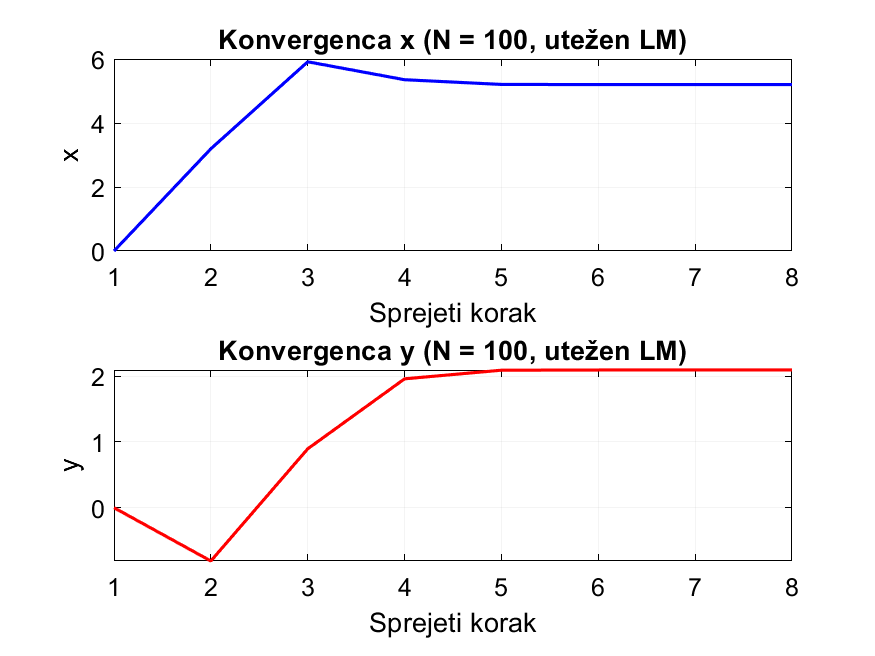
\includegraphics[width=0.9\textwidth]{figs/main_convergence_plot.png}
    \caption{Konvergenca parametrov $x$ in $y$ po sprejetih korakih utežene LM optimizacije pri $N=100$.}
    \label{fig:conv_main}
\end{figure}

Slika~\ref{fig:geom_main} prikazuje geometrijo problema: bazne postaje, ročno narisane krožnice z radiji $\bar{d}_i$, pot optimizacije ter obe končni oceni. Krožnice se zaradi šuma ne sekajo v eni točki, obe oceni pa ležita v območju njihovega ``skoraj-presečišča''.

\begin{figure}[H]
    \centering
    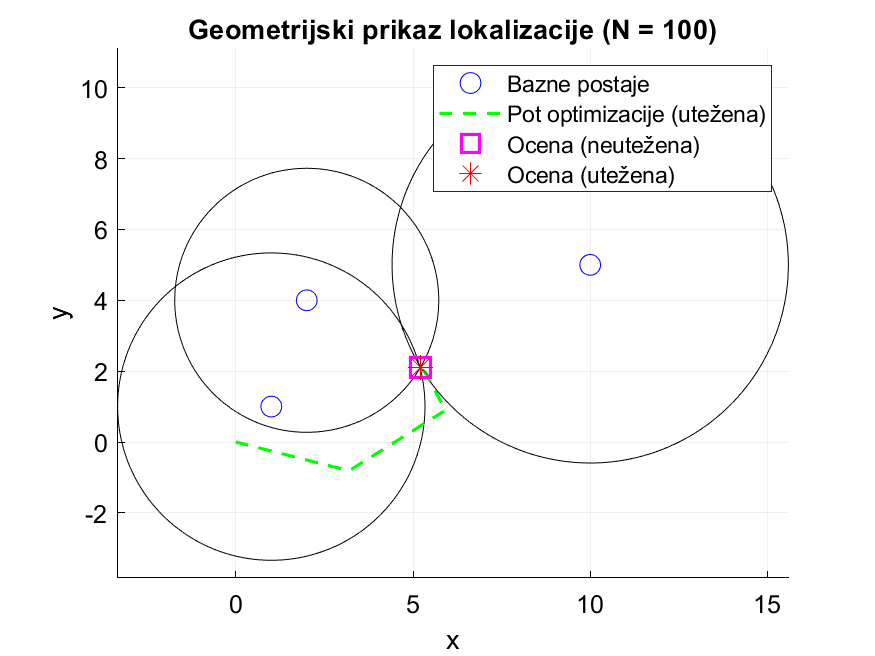
\includegraphics[width=0.82\textwidth]{figs/main_geometry_plot.png}
    \caption{Geometrijski prikaz lokalizacije telefona za $N=100$ z ročno narisanimi krožnicami ter neuteženo in uteženo oceno.}
    \label{fig:geom_main}
\end{figure}

\subsection{Monte Carlo analiza vpliva števila meritev}
Tabela~\ref{tab:results} povzema rezultate $M=100$ neodvisnih ponovitev za vsak $N$.

\begin{table}[H]
\centering
\begin{tabular}{|c|c|c|c|c|c|}\hline
\v{S}tevilo meritev (N) & Povpr. $x$ & Povpr. $y$ & Povpr. \v{s}t. iteracij & MC Var($x$) & MC Var($y$) \\\hline
1 & 5.1911 & 2.0716 & 9.6 & 0.010771 & 0.084259 \\
5 & 5.1922 & 2.0809 & 8.5 & 0.002071 & 0.016052 \\
10 & 5.1969 & 2.0986 & 8.2 & 0.000981 & 0.007555 \\
50 & 5.1996 & 2.1012 & 7.8 & 0.000198 & 0.001808 \\
100 & 5.1994 & 2.0990 & 7.6 & 0.000104 & 0.000779 \\
\hline\end{tabular}

\caption{Monte Carlo rezultati za različne vrednosti števila meritev $N$ ($M=100$ ponovitev na vsak $N$, neutežena varianta).}
\label{tab:results}
\end{table}

Povprečne ocene so za vse $N$ praktično enake (okoli $(5.19,\,2.10)$) -- povprečenje čez $M$ ponovitev odstrani naključni raztros posamezne ponovitve. Bistvena razlika med vrednostmi $N$ je v MC varianci končnih ocen, ki z naraščajočim $N$ strmo pada: $\operatorname{Var}(\hat{x})$ od $0.010771$ pri $N=1$ do $0.000104$ pri $N=100$, $\operatorname{Var}(\hat{y})$ od $0.084259$ do $0.000779$. Povprečno število iteracij rahlo pada z $N$ (od $9.6$ pri $N=1$ do $7.6$ pri $N=100$): manj šumni podatki dajo bolj konsistentne reziduale in nekoliko lažjo optimizacijo, konvergenca pa je hitra v vseh primerih.

Slika~\ref{fig:mc_scatter} raztros prikaže neposredno: vsak oblak točk so končne ocene $100$ neodvisnih ponovitev pri danem $N$. Krčenje oblakov z naraščajočim $N$ je vizualni prikaz padanja variance iz tabele~\ref{tab:results}.

\begin{figure}[H]
    \centering
    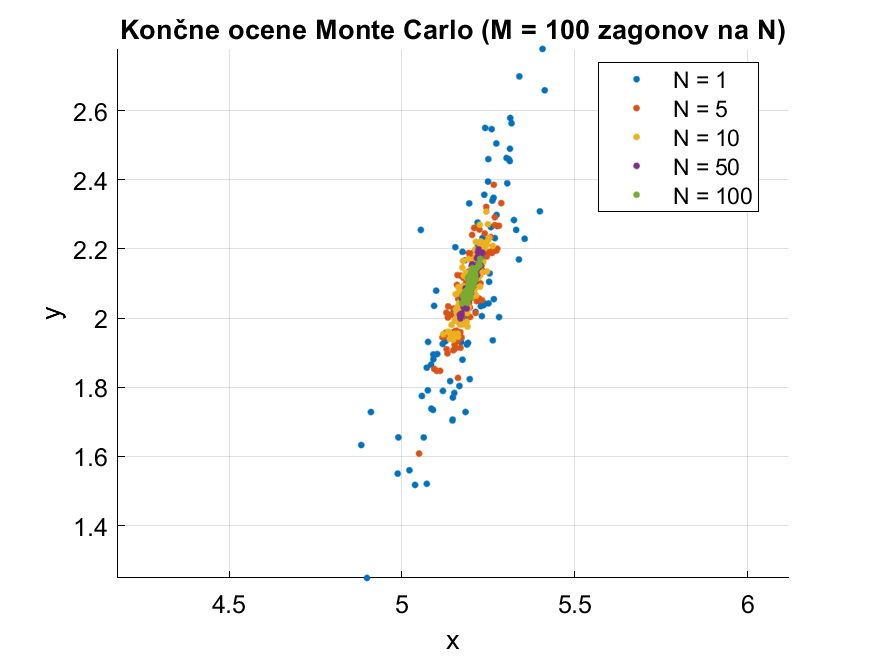
\includegraphics[width=0.8\textwidth]{figs/mc_scatter.png}
    \caption{Oblaki končnih Monte Carlo ocen za različne $N$. Z večanjem $N$ se raztros ocen vidno krči.}
    \label{fig:mc_scatter}
\end{figure}

Sliki~\ref{fig:var_vs_n} in~\ref{fig:iter_vs_n} prikazujeta MC varianco in povprečno število iteracij v odvisnosti od $N$.

\begin{figure}[H]
    \centering
    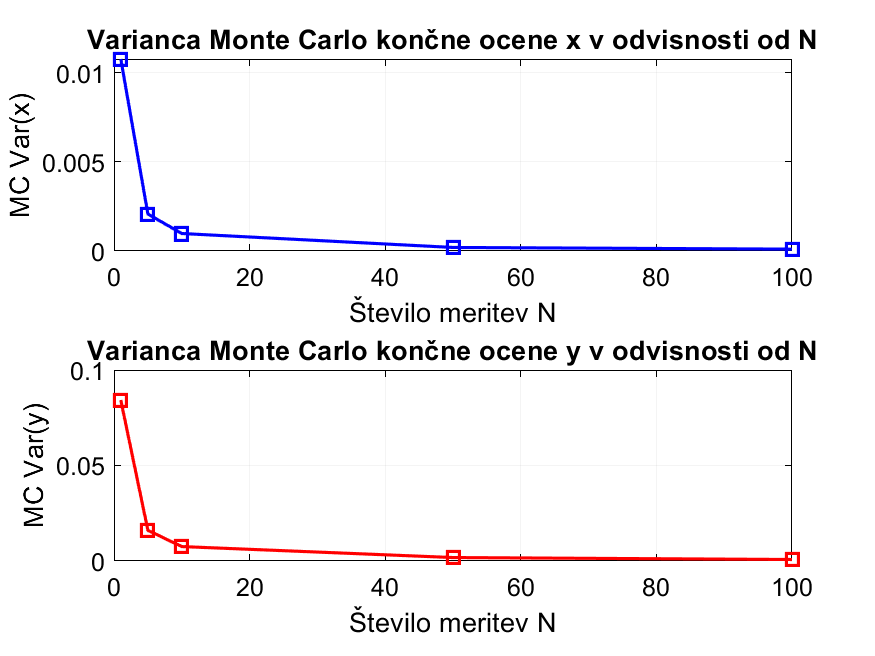
\includegraphics[width=0.9\textwidth]{figs/variance_vs_measurements.png}
    \caption{Monte Carlo varianca končnih ocen $\hat{x}$ in $\hat{y}$ v odvisnosti od števila meritev $N$. Varianca z naraščajočim $N$ pada v skladu z zakonom $1/N$.}
    \label{fig:var_vs_n}
\end{figure}

\begin{figure}[H]
    \centering
    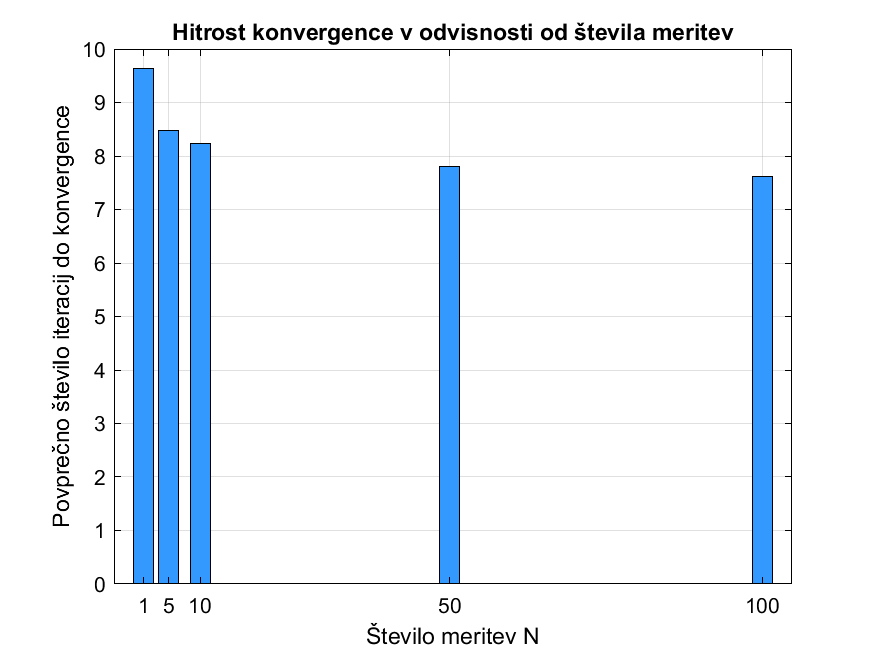
\includegraphics[width=0.8\textwidth]{figs/iterations_vs_measurements.png}
    \caption{Povprečno število iteracij do konvergence glede na število meritev $N$.}
    \label{fig:iter_vs_n}
\end{figure}

\subsection{Primerjava uteženega in neuteženega pristopa}
Tabela~\ref{tab:wls} povzema primerjavo obeh pristopov čez $M=100$ neodvisnih ponovitev pri $N=100$, pri čemer sta v vsaki ponovitvi obe varianti uporabili iste podatke.

\begin{table}[H]
\centering
\begin{tabular}{|l|c|c|c|c|c|c|}\hline
Varianta & Povpr. $x$ & Povpr. $y$ & Var($x$) & Var($y$) & Std($x$) & Std($y$) \\\hline
Neute\v{z}eno & 5.1971 & 2.0927 & 0.000112 & 0.000863 & 0.0106 & 0.0294 \\
Ute\v{z}eno (WLS) & 5.1983 & 2.0981 & 0.000054 & 0.000213 & 0.0074 & 0.0146 \\
\hline\end{tabular}

\caption{Primerjava neuteženih in uteženih (WLS) najmanjših kvadratov čez $M=100$ ponovitev pri $N=100$.}
\label{tab:wls}
\end{table}

Slika~\ref{fig:wls_scatter} prikazuje oba oblaka končnih ocen. Uteženi oblak je vidno bolj zgoščen od neuteženega, obe povprečji pa sovpadata.

\begin{figure}[H]
    \centering
    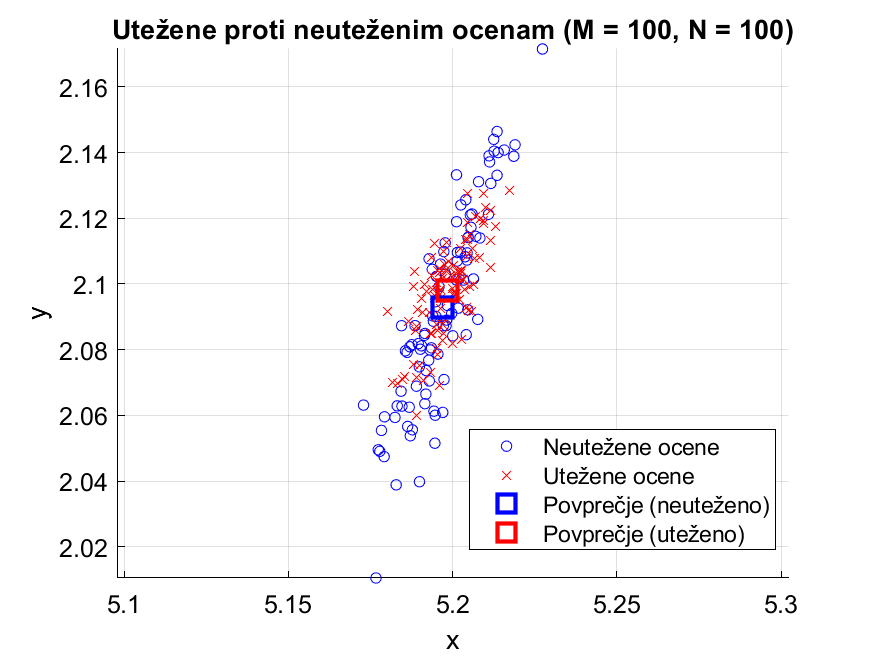
\includegraphics[width=0.8\textwidth]{figs/weighted_vs_unweighted.png}
    \caption{Oblaka končnih ocen neutežene in utežene optimizacije ($M=100$, $N=100$). Uteženje raztros ocen občutno zmanjša.}
    \label{fig:wls_scatter}
\end{figure}

\section{Analiza in interpretacija rezultatov}
\label{sec:analiza}

\subsection{Kvantitativna potrditev zakona $1/N$}
Enačba~\eqref{eq:oneOverN} napove, da mora MC varianca ocene pasti obratno sorazmerno s številom meritev: pri $100$-krat večjem $N$ pričakujemo $100$-krat manjšo varianco. Razmerji izmerjenih varianc med skrajnima vrednostma $N$ znašata
\[
\frac{\operatorname{Var}(\hat{x})\big|_{N=1}}{\operatorname{Var}(\hat{x})\big|_{N=100}} = \frac{0.010771}{0.000104} \approx 104,
\qquad
\frac{\operatorname{Var}(\hat{y})\big|_{N=1}}{\operatorname{Var}(\hat{y})\big|_{N=100}} = \frac{0.084259}{0.000779} \approx 108,
\]
kar se zelo dobro ujema s teoretično napovedjo $N = 100$. Razlog je preprost: povprečje $N$ neodvisnih meritev ima varianco $\sigma^2/N$, končna ocena pozicije pa je gladka funkcija teh povprečij, zato podeduje isti faktor $1/N$. Manjši odstopanji od točne vrednosti $100$ ($\approx 104$ oziroma $\approx 108$) sta pričakovana posledica končnega števila ponovitev ($M=100$) -- tudi sama MC ocena variance je namreč naključna količina s svojim raztrosom. Enak trend potrjujejo vmesne vrednosti $N$ v tabeli~\ref{tab:results} in krčenje oblakov na sliki~\ref{fig:mc_scatter}.

\subsection{Učinek uteževanja z varianco meritev}
Primerjava v tabeli~\ref{tab:wls} pokaže, da uteženje po enačbi~\eqref{eq:W} raztros končnih ocen občutno zmanjša: varianca $\hat{x}$ pade z $0.000112$ na $0.000054$ (faktor $\approx 2.1$), varianca $\hat{y}$ z $0.000863$ na $0.000213$ (faktor $\approx 4.1$); standardna odklona se zmanjšata s $0.0106$ na $0.0074$ oziroma z $0.0294$ na $0.0146$. Povprečji obeh pristopov sovpadata ($(5.1971,\,2.0927)$ proti $(5.1983,\,2.0981)$), kar pomeni, da uteženje ne vnaša pristranskosti, temveč zgolj zmanjšuje občutljivost ocene na šum najmanj zanesljive postaje. Dobitek je največji v smeri $y$, kjer ima nezanesljiva postaja 2 (varianca $0.1013$, tabela~\ref{tab:station_var}) največji vpliv na geometrijo presečišča. To je pričakovano: WLS informacijo o različni zanesljivosti postaj izkoristi, neuteženi pristop pa jo zavrže.

Pri glavni lokalizaciji je utežena varianta potrebovala $13$ iteracij, neutežena pa $7$. To ni pomanjkljivost uteženega pristopa. Uteži $1/\sigma_i^2$ (od $\approx 10$ za postajo 2 do $\approx 370$ za postajo 3) močno spremenijo skaliranje kriterijske funkcije in ukrivljenost njene površine, zato isti začetni $\lambda_0$ ustreza drugačnemu razmerju med dušenjem in Gauss--Newtonovim korakom -- metoda naredi nekaj več krajših, previdnejših korakov. Vsaka iteracija je računsko trivialna (rešitev sistema $2\times 2$), obe varianti konvergirata v nekaj deset milisekundah, kakovost končne ocene pa je pri uteženi varianti boljša; nekaj dodatnih iteracij je zanemarljiva cena za približno prepolovljen standardni odklon.

\subsection{Vloga logike sprejmi/zavrni}
LM iteracija z logiko sprejmi/zavrni po sprejetih korakih garantira strogo padanje kriterija $J = \mathbf{F}^T\mathbf{W}\mathbf{F}$, s čimer je izključena možnost, da bi metoda sprejela korak, ki oceno poslabša. Brezpogojno sprejemanje korakov te lastnosti nima: položaj se posodobi tudi ob predolgem koraku, prilagoditev $\lambda$ pa nastopi šele naknadno. Hkrati velja poudariti, kar smo videli na sliki~\ref{fig:conv_main}: garancija se nanaša na kriterij, ne na posamezne koordinate. Začasni zavoj koordinate $y$ v negativno območje je sprejet korak, ki je kriterij dejansko zmanjšal, in je zato povsem legitimen del konvergence, ne numerična napaka. V praksi se je varovalka $\lambda \le 10^{10}$ izkazala za nepotrebno (nikoli ni bila sprožena), a je nujen del robustne implementacije.

\section{Zaključek}
V nalogi smo implementirali metodo nelinearnih najmanjših kvadratov z Levenberg--Marquardtovo optimizacijo za lokalizacijo mobilnega telefona iz šumnih meritev razdalj do treh baznih postaj, z metodološko doslednim pristopom: kriterijska funkcija $J=\mathbf{F}^T\mathbf{W}\mathbf{F}$ z utežmi $1/\sigma_i^2$ upošteva izmerjeno varianco meritev posameznih postaj, LM iteracija z logiko sprejmi/zavrni garantira monotono padanje kriterija, negotovost ocene pa je ovrednotena s pravilno mero -- Monte Carlo varianco končnih ocen čez neodvisne ponovitve.

Glavna lokalizacija pri $N=100$ je dala uteženo oceno položaja telefona
\[
(x,y) = (5.2009,\; 2.0948)
\]
v $13$ iteracijah (neuteženo $(5.2050,\;2.1111)$ v $7$ iteracijah). Monte Carlo analiza je kvantitativno potrdila teoretični zakon $1/N$: varianca ocene je pri $N=100$ približno $104$-krat (za $x$) oziroma $108$-krat (za $y$) manjša kot pri $N=1$. Primerjava pristopov je pokazala, da uteženje z inverznimi variancami meritev raztros ocene zmanjša za faktor $2$ do $4$ pri nespremenjenem povprečju, torej se splača vselej, ko lahko varianco meritev ocenimo. Skupaj rezultati potrjujejo, da je pravilno zastavljena metoda nelinearnih najmanjših kvadratov -- z uteževanjem, nadzorovanim sprejemanjem korakov in korektno statistično oceno negotovosti -- zanesljivo orodje za tovrstne lokalizacijske probleme.

\newpage
\section*{Priloga: Koda}
V prilogi je navedena celotna skripta, ki izvede glavno lokalizacijo (neuteženo in uteženo), Monte Carlo analizo vpliva števila meritev, primerjavo pristopov ter izriše vse slike in izdela vse tabele. Levenberg--Marquardtova metoda z logiko sprejmi/zavrni je implementirana v lokalni funkciji \texttt{run\_lm} na dnu skripte.

\lstinputlisting[language=Matlab]{vaja1.m}

\end{document}
